\documentclass[a4paper,12pt]{report}
\usepackage{amsmath,amsfonts,amssymb,enumerate,graphicx,fancyhdr,times}
\usepackage{tabularx,float,xspace,float,caption,setspace}
\usepackage[top=2.5cm, left = 3cm, right = 1.5cm, bottom = 2.5cm]{geometry}
\usepackage[utf8]{inputenc}

\pagestyle{fancyplain}
\fancyhf{}
\renewcommand{\headrulewidth}{0px}
\fancyfoot[R]{\thepage}
\parindent 0px

\begin{document}

\begin{titlepage}

	\centering

	
\includegraphics[width=3cm, keepaspectratio]{cuet.png} \par \vspace{0.5cm}
	\begin{Large}
		CHITTAGONG UNIVERSITY OF ENGINEERING \& TECHNOLOGY
	\end{Large}
	\par
	\vspace{.5cm}
	{DEPARTMENT OF COMPUTER SCIENCE AND ENGINEERING}
\vspace{1cm}

	\raisebox{-\baselineskip}{\rule{\textwidth}{1px}}
	\rule{\textwidth}{1px}

\vspace{0.2cm}
{\Large{{EXPERIMENT NAME}}}\par \vspace{0.3cm}
\huge{{Completion of other pages and initialization of the database of ``SmartHaat" Website}}
	\rule{\textwidth}{2px}

\vspace{0.5cm}

	\normalsize
\begin{tabular}{cl}
COURSE CODE        & : CSE 326                          \\
COURSE NAME        & : INTERNET PROGRAMMING (SESSIONAL) \\
EXPERIMENT NO      & : 05                               \\
DATE OF SUBMISSION & : 19 -- 07 -- 2023
\end{tabular}
\vspace{0.5cm}

	\parbox[l]{9cm}{
		\begin{center}
			submitted by
		\end{center}

		\begin{tabular}{cl}
			MD AKIB HASAN        & $(1904015)$ \\
K.M. MAHABUB HOSSAIN & $(1904017)$ \\
			SADMAN RAHMAN ANANTA & $(1904020)$ \\
		\end{tabular}
	}
	\parbox[r]{7cm}{
		\vspace{1cm}
		\begin{center}
			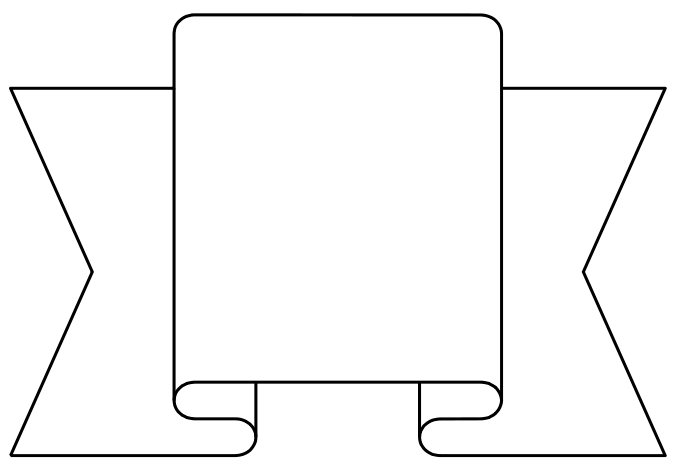
\includegraphics[width=4cm, keepaspectratio]{remarks.png}
			\captionof*{figure}{REMARKS}
		\end{center}
	}

	\vspace{0.5cm}
	supervised by

	\parbox[l]{8cm}{\begin{center}

			SABIHA ANAN\\
\footnotesize{Assistant Professor\\
				Department of CSE, CUET}
		\end{center}
	}
	\parbox[r]{8cm}{\begin{center}

			MD RASHADUR RAHMAN\\
\footnotesize{Lecturer \\
				Department of CSE, CUET}
		\end{center}
	}

	\vfill
\end{titlepage}


\onehalfspacing

\section*{Experiment Name}
Completion of other pages and initialization of the database of ``SmartHaat" Website.
\section*{Objectives}
\begin{itemize}
\item Building Shipment and other pages.
\item Improvements in showing data of products.
\item Implementing database and connection establishment.
\end{itemize}
\section*{Description}
A websites compatibility and efficiency depends on quick response to the user and providing them hassle-free service. Therefore, we implemented lots of modules as card and other way instead of new pages.
\begin{figure}[H]
\centering
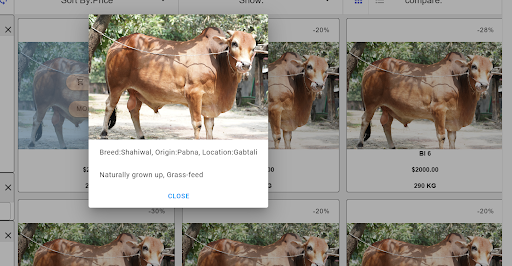
\includegraphics[keepaspectratio, width=12cm]{pop_up.png}
\caption{Pop up view of see more page}
\label{popup}
\end{figure}
The pop-up view is created  to show the more information about the product. So, the user can browse the products without changing the page and follow its specification as well as bookmark and cart it.

The shipping page includes receivers name, location, authentication and other the shipping information for an order. It is shown after confirming order. And other shipment status are shown in the user's page where they can track their previous orders too.
\begin{figure}[H]
\centering
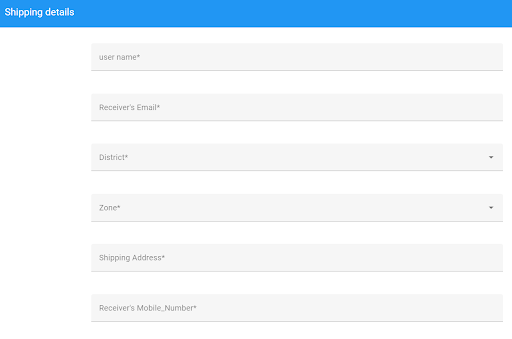
\includegraphics[keepaspectratio, width=12cm]{shipping.png}
\caption{Shipping page}
\label{shipping}
\end{figure}
Like any other e-commerce website, our website requires a database system to track users information, seller and theirs products' information, selling status and other authenticating information. To incorporate with the Vue framework, a general database system with rest API are initialized. Where we need to create APIs to communicate from webpage with database.
\begin{figure}[H]
\centering
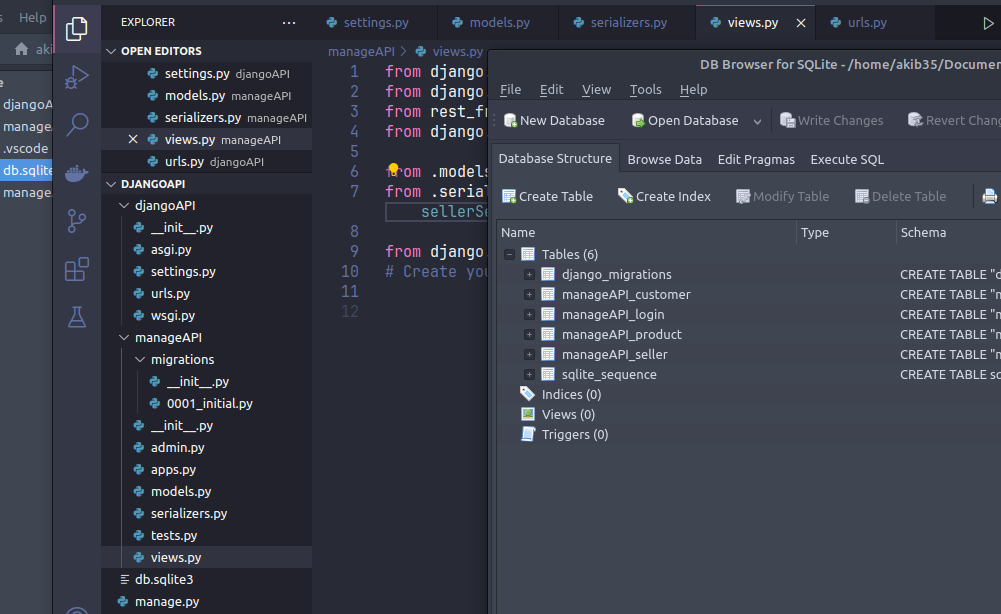
\includegraphics[keepaspectratio, width=12cm]{db.png}
\caption{Database initialization}
\label{db}
\end{figure}
Here the main tables to perform a static view of our website are created initially which can be seen in figure \ref{db}. It contains many tables such as products, seller, customer and login tables with necessary relations.


\section*{Development Platforms}
The frameworks and language platforms we used --
\begin{itemize}
	\item HTML
	\item CSS
\item JavaScript
	\item VUE
\item Django REST API
\item Sqlite3
\end{itemize}

\section*{Conclusion}
A website needs to have less distraction and in time delivery of the needs to the customer. Therefore, easy and quick responsive pages are built for our website.
This week we improved our home page with few more functionalities and features. The shipment page took a bit of difficulty, but it was solved finally. And the database we created is in initial state and the data can't be accessed without proper APIs and that's why the actual functions are not available.
\end{document}
